\chapter{分布式对象存储系统管控平台详细设计与实现}

本章将深入介绍分布式对象存储系统管控平台的详细设计,根据微服务划分的功能模块,对每一模块的设计和实现过程进行细致的梳理,最后,针对本系统涉及到的数据库表
进行了全面的介绍。

\section{注册认证模块设计与实现}

本系统的认证模块使用了Spring Security框架和JWT(JSON Web Token)技术相结合的方式实现\cite{k256eji}。Spring Security是Spring框架体系中专门处理安全管理
方面的框架,它拥有功能性强、扩展性高等优点,能够为系统提供全面的安全保障。而JWT则是一种用于跨域认证的标准化解决方案,具有安全、灵活、易用等特
点,能够有效地实现认证功能。因此,本系统的注册认证模块选择了将这两种技术进行整合,以便更好地保障系统的安全性和可扩展性。

(1)用户注册子模块

\begin{figure}[htb]
    \centering
    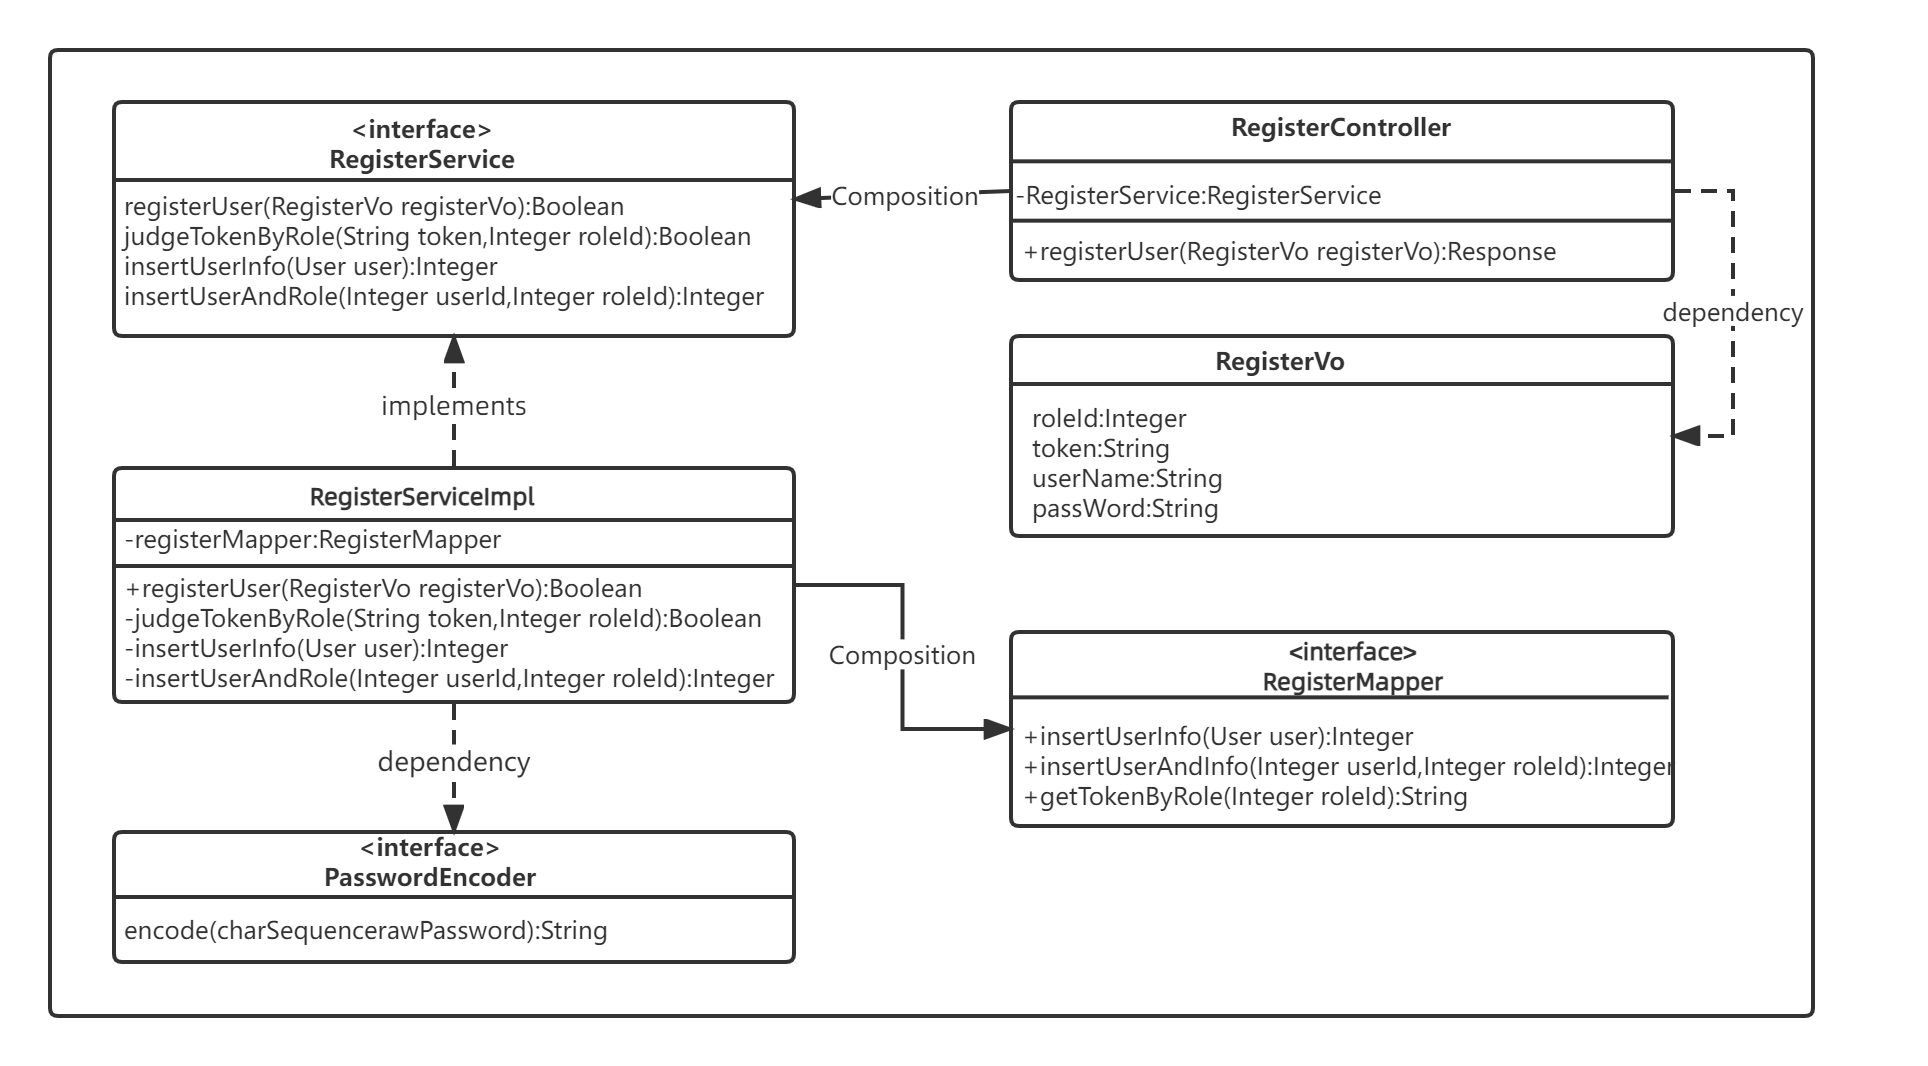
\includegraphics[width=1\textwidth]{my_figures/chapter5/用户注册子模块UML类图.png}
    \caption{用户注册子模块UML类图}
    \label{fig:用户注册子模块UML类图}
%     \note{注:图注的内容不宜放到图题中。}
\end{figure}

用户注册子模块的UML类图如图\ref{fig:用户注册子模块UML类图}所示。该子模块主要涉及六个类,分别是RegisterController、RegisterVo、RegisterService、RegisterServiceImpl、RegisterMapper和PasswordEncoder。
其中RegisterController包含一个属性类RegisterService和一个方法registerUser,registerUser接收一个参数RegisterVo,其中封装了来自前端的注册信息,包括roleId、userName、
password、email等,它们分别表示角色编号、用户名、密码和邮箱。RegisterService是一个接口,其实现类RegisterServiceImpl有方法registerUser、insertUserAndRole等方法,专门
用来插入用户和角色的绑定信息。RegisterMapper也是一个接口,不需要实现类,用来将注册信息存入数据库。PasswordEncoder接口只有一个encode方法,主要是为了给密码编码。



根据类图我们可以进一步绘制出该子模块的UML时序图,如图\ref{fig:用户注册子模块UML时序图}所示。当用户点击注册按钮时,注册请求会从前端发送到控制器RegisterController,RegisterController会调用registerUser方法,
registerUser需要一个RegisterVo参数,然后RegisterController会调用RegisterService的实现类RegisterServiceImpl的方法,准备插入用户信息。在插入之前,会调用
PasswordEncoder接口中的encode方法对密码进行编码,因为密码必须通过特殊处理后才可存入数据库。然后利用RegisterMapper接口中的registerUser、insertUserAndRole等方法将用户名、
密码等信息插入到数据库。值得注意的是,RegisterMapper接口不需要实现类,由于利用了mybatis,只要在开发相关的接口后填写对应配置文件即可。

\begin{figure}[htb]
    \centering
    \includegraphics[width=1\textwidth]{my_figures/chapter5/用户注册子模块UML时序图.png}
    \caption{用户注册子模块UML时序图}
    \label{fig:用户注册子模块UML时序图}
%     \note{注:图注的内容不宜放到图题中。}
\end{figure}

(2)用户登录子模块

\begin{figure}[htb]
    \centering
    \includegraphics[width=1\textwidth]{my_figures/chapter5/用户登录子模块UML类图.png}
    \caption{用户登录子模块UML类图}
    \label{fig:用户登录子模块UML类图}
%     \note{注:图注的内容不宜放到图题中。}
\end{figure}

用户登录子模块的UML类图如图\ref{fig:用户登录子模块UML类图}所示。该子模块主要包含七个类,分别是LoginFilter、AuthenticationManager、UserDetailsService、UserDetails、UserDetailsServiceImpl、SecurityUser和
PasswordEncoder类。其中,LoginFilter包含一个属性类AuthenticationManager和三个方法attempAuthentication、sucessfulAuthentication,unsucessfulAuthentication。
AuthenticationManager中有一个属性类UserDetailsService和一个方法authenticate,方法接收Authentication参数,UserDetailsService是一个接口,其含有方法loadUserByUsername,
其参数是username,返回值为UserDetails,UserDetails也是一个接口,其用来获取用户名、密码以及token,其实现类为SecurityUser。loadUserByUsername方法在UserDetailsService的
实现类UserDetailsServiceImpl中被具体实现,该实现类含有两个属性类,分别是PasswordEncoder和UserMapper。PasswordEncoder含有encode方法和matches方法,分别进行密码的编码和
比对。

\begin{figure}[htb]
    \centering
    \includegraphics[width=1\textwidth]{my_figures/chapter5/用户登录子模块UML时序图.png}
    \caption{用户登录子模块UML时序图}
    \label{fig:用户登录子模块UML时序图}
%     \note{注:图注的内容不宜放到图题中。}
\end{figure}


根据类图我们可以进一步绘制出该子模块的UML时序图,如图\ref{fig:用户登录子模块UML时序图}所示。当用户点击登录按钮时,LoginFilter获取到用户的用户名和密码,然后在AuthenticationManager
中对用户名和密码进行验证,在验证前,需要先从调用UserDetailsService中的方法去获取用户信息,通过UserMapper去数据库取到所有用户名和密码,将密码进行编码并进行逐一比对,将信息封装
到UserDetails中,返回给AuthenticationManager,AuthenticationManager对密码进行验证,验证完成后,向LoginFilter返回Authentication。至此,用户的用户名和密码均验证成功,用户
成功登录。




(3)身份认证子模块

\begin{figure}[htb]
    \centering
    \includegraphics[width=1\textwidth]{my_figures/chapter5/身份认证子模块UML类图.png}
    \caption{身份认证子模块UML类图}
    \label{fig:身份认证子模块UML类图}
%     \note{注:图注的内容不宜放到图题中。}
\end{figure}

身份认证子模块的UML类图如图\ref{fig:身份认证子模块UML类图}所示。该子模块主要有思格雷,分别是TokenValidAuthentication、TokenAuthentication、TokenAuthenticationImpl和JWTUtil。
其中TokenValidAuthentication中含有一个属性类TokenAuthentication和一个方法judgeToken。方法judgeToken接收一个HttpServletRequest的参数,从里面可以获取到当前请求的token。
TokenAuthentication是一个接口,其中含有两个方法,分别是getTokenByAuthentication和judgeTokenByExpire,它们接收的参数类型都是Authentication,Authentication中含有当前请求的
token,TokenAuthentication通过实现类TokenAuthenticationImpl来实现这两个方法,实现类中还有一个方法为setTokenInvalid,用来将token置为无效。JWTUtil中有一个方法
getUserInfoFromToken,它将token作为参数用来得到用户信息。

\begin{figure}[htb]
    \centering
    \includegraphics[width=1\textwidth]{my_figures/chapter5/身份认证子模块UML时序图.png}
    \caption{身份认证子模块UML时序图}
    \label{fig:身份认证子模块UML时序图}
%     \note{注:图注的内容不宜放到图题中。}
\end{figure}

根据类图我们可以进一步绘制出该子模块的UML时序图,如图\ref{fig:身份认证子模块UML时序图}所示。当用户登录后点击不同的页面时,系统都会对其token进行认证。TokenValidAuthentication
会从每个请求的header取出token,在TokenAuthenticationImpl中去判断token是否过期,如果token过期,则将JWTUtil中的token设为无效,而且这时会跳转到登录页面,要求用户重新进行登录。
登录成功后,会重新生成新的token,将新的token返回给TokenValidAuthentication,TokenValidAuthentication验证到新的token后,就会认证成功,此时页面自动跳转到用户需要访问的
页面。




\section{权限控制模块设计与实现}

(1)权限管理子模块

\begin{figure}[htb]
    \centering
    \includegraphics[width=1\textwidth]{my_figures/chapter5/权限管理子模块UML类图.png}
    \caption{权限管理子模块UML类图}
    \label{fig:权限管理子模块UML类图}
%     \note{注:图注的内容不宜放到图题中。}
\end{figure}

权限管理子模块的UML类图如图\ref{fig:权限管理子模块UML类图}所示。该子模块主要包含五个类,分别是PermissionController、PermissionService、PermissionServiceImpl、PermissionMapper
和PermissionVo。PermissionController类中包含一个属性类PermissionService和四个方法getPermissionList、updatePermission、insertPermission和deletePermission,它们分别
负责权限的查询、修改、创建和删除,接收的参数类型为PermissionVo,PermissionVo包含permissionId、permissionName和token,即对应权限编号、权限名称以及令牌。PermissionService
中含有与PermissionController同名的方法,它们在实现类PermissionServiceImpl中被具体实现,该实现类还含有一个属性类PermissionMapper,PermissionMapper主要用来操作数据库中与权限
相关的数据。

\begin{figure}[htb]
    \centering
    \includegraphics[width=1\textwidth]{my_figures/chapter5/权限管理子模块UML时序图.png}
    \caption{权限管理子模块UML时序图}
    \label{fig:权限管理子模块UML时序图}
%     \note{注:图注的内容不宜放到图题中。}
\end{figure}

根据类图我们可以进一步绘制出该子模块的UML时序图,如图\ref{fig:权限管理子模块UML时序图}所示。当系统管理员在权限管理页面进行创建、删除、修改、查看权限等操作时,这些请求会从前端发送
到控制器PermissionController,PermissionController首先获取到token,将token传给TokenValidAuthentication进行验证,验证通过后,将对系统中的权限进行相关操作,通过调用
PermissionService接口中的方法来完成这些步骤。PermissionService会调用PermissionMapper中的具体接口去对数据库中的权限信息进行增删改查的操作。完成后,系统会将完成状态信息或返
数据返回到前端页面进行显示。

(2)角色管理子模块

\begin{figure}[htb]
    \centering
    \includegraphics[width=1\textwidth]{my_figures/chapter5/角色管理子模块UML类图.png}
    \caption{角色管理子模块UML类图}
    \label{fig:角色管理子模块UML类图}
%     \note{注:图注的内容不宜放到图题中。}
\end{figure}

角色管理子模块的UML类图如图\ref{fig:角色管理子模块UML类图}所示。该子模块主要包含七个类,分别是RoleController、RoleService、RoleServiceImpl、RoleMapper、RoleVo、
RolePermissionVo和RoleUserVo。RoleController中含有一个属性类RoleService和六个方法,分别是getRoleList、distributeRoleAndPermission、
deletePermissionByRole、insertRoleAndPermission和distributeRoleAndUser,它们都是关于角色查询和角色分配的相关接口。在RoleService也有相同的方法,由于RoleService也是一个
接口类,所以这些方法在其实现类RoleServiceImpl中实现,该实现类中有一个属性类RoleMapper,该类也包含了以上方法。RoleVo、RolePermissionVo和RoleUserVo类分别是角色信息、角色权限
关联信息和角色用户关联信息。

\begin{figure}[htb]
    \centering
    \includegraphics[width=1\textwidth]{my_figures/chapter5/角色管理子模块UML时序图.png}
    \caption{角色管理子模块UML时序图}
    \label{fig:角色管理子模块UML时序图}
%     \note{注:图注的内容不宜放到图题中。}
\end{figure}

根据类图我们可以进一步绘制出该子模块的UML时序图,如图\ref{fig:角色管理子模块UML时序图}所示。当系统管理员想要进行角色分配时,该请求从前端传到RoleController,RoleController会向将
token传给TokenValidAuthentication进行token验证,验证成功后,RoleController获取角色和权限或用户的关联信息,调用RoleService的distributeRoleAndPermission或
distributeRoleAndUser进行操作,RoleService进一步调用RoleMapper中的distributeRoleAndPermission或distributeRoleAndUser方法将相关信息写入数据库中。完成后,返回完成状态,
在前端页面进行显示。


(3)网关鉴权子模块

\begin{figure}[htb]
    \centering
    \includegraphics[width=1\textwidth]{my_figures/chapter5/网关鉴权子模块UML类图.png}
    \caption{网关鉴权子模块UML类图}
    \label{fig:网关鉴权子模块UML类图}
%     \note{注:图注的内容不宜放到图题中。}
\end{figure}

网关鉴权子模块的UML类图如图\ref{fig:网关鉴权子模块UML类图}所示。该子模块主要包含四个类,分别是GatewayAuthentication、PermissionAuthentication、PermissionAuthenticationImpl
和Permission。其中,GatewayAuthentication类含有一个属性类PermissionAuthentication和一个方法judgePermission,judgePermission接收一个HttpServletRequest类型的参数。
PermissionAuthentication是一个接口类,其中含有三个方法,分别是getUsernameByAuthentication、getPermissionListByUername和judgePermission,它们的参数都是Authenticationl
类型。PermissionAuthentication中的方法在其实现类PermissionAuthenticationImpl中实现,这些方法会涉及到Permission类,该类中的属性包括permissionId和permissionName,即权限
编号和权限名称。

\begin{figure}[htb]
    \centering
    \includegraphics[width=1\textwidth]{my_figures/chapter5/网关鉴权子模块UML时序图.png}
    \caption{网关鉴权子模块UML时序图}
    \label{fig:网关鉴权子模块UML时序图}
%     \note{注:图注的内容不宜放到图题中。}
\end{figure}


根据类图我们可以进一步绘制出该子模块的UML时序图,如图\ref{fig:网关鉴权子模块UML时序图}所示。当用户点击任何页面请求时,网关都要对该请求进行鉴权,GatewayAuthentication会从
请求的header中拿到token和URL,PermissionAuthentication通过token拿到用户名,然后根据拿到的用户名调用PermissionService的接口查询对应的权限列表,PermissionService进一步调用
PermissionMapper中的接口从数据库中取出用户对应的所有权限。PermissionAuthentication将在返回的权限列表中查找从请求中拿到的URL,如果URL在权限列表中,则说明该用户拥有此接口的
访问的权限,用户可正常操作;否则,用户没有该权限,返回无权访问的错误,前端页面显示操作非法。



\section{策略控制模块设计与实现}

(1)用户管理子模块

\begin{figure}[htb]
    \centering
    \includegraphics[width=1\textwidth]{my_figures/chapter5/用户管理子模块UML类图.png}
    \caption{用户管理子模块UML类图}
    \label{fig:用户管理子模块UML类图}
%     \note{注:图注的内容不宜放到图题中。}
\end{figure}

用户管理子模块的UML类图如图\ref{fig:用户管理子模块UML类图}所示。该子模块主要包含六个类,分别是IdentityController、IdentityService、IdentityServiceImpl、IdentityMapper、 
AliioClient和UserVo。其中,IdentityController中含有一个属性类IdentityService和四个方法,分别是getUserList、updateUser、insertUser和deleteUser,它们接收一个User类的参
数UserVo,UserVo中含有用户有关的信息,如userId、userName、password和email,即用户编号、用户名、密码和邮箱。IdentityService中有上述的同名方法,这些方法在其实现类
IdentityServiceImpl被实现,该实现类中含有一个属性类IdentityMapper,该接口类也含有上述同样的方法。AliioClient类中也同样含有这些方法,该类是由对象存储系统AliIO提供的API,
主要负责对存储服务器进行相关操作。

\begin{figure}[htb]
    \centering
    \includegraphics[width=1\textwidth]{my_figures/chapter5/用户管理子模块UML时序图.png}
    \caption{用户管理子模块UML时序图}
    \label{fig:用户管理子模块UML时序图}
%     \note{注:图注的内容不宜放到图题中。}
\end{figure}

根据类图我们可以进一步绘制出该子模块的UML时序图,如图\ref{fig:用户管理子模块UML时序图}所示。当管理员在进行用户的创建、删除、修改和查询等操作时,这里以创建用户为例。
IdentityController收到创建用户的操作请求后,首先获取新增用户的信息,然后调用IdentityService中的insertUser方法将用户信息插入系统,IdentityService进一步调用IdentityMapper
的insertUser方法将用户信息存入数据库中。同时,IdentityService还会调用AliIOClient中的createUser方法在存储服务器中创建同名的系统用户。
然后,存储服务器会将完成状态返回给IdentityService类,IdentityService类继续将完成状态返回给IdentityController,最后显示在前端页面。


(2)策略管理子模块



策略管理子模块的UML类图如图\ref{fig:策略管理子模块UML类图}所示。该子模块主要包含六个类,分别是PolicyController、PolicyService、PolicyServiceImpl、PolicyMapper、 
AliioClient和PolicyVo。其中,PolicyController中含有一个属性类PolicyService和四个方法,分别是getPolicyList、updatePolicy、insertPolicy和deletePolicy,
它们接收一个Policy类的参数PolicyVo,PolicyVo中含有策略有关的信息,如policyId、policyName、state和operateList,即策略编号、策略名称、状态和操作列表。
PolicyService中有上述的同名方法,这些方法在其实现类
PolicyServiceImpl被实现,该实现类中含有一个属性类PolicyMapper,该接口类也含有上述同样的方法。AliioClient类中也同样含有这些方法,该类是由对象存储系统AliIO提供的API,
主要负责对存储服务器进行相关操作。

\begin{figure}[htb]
    \centering
    \includegraphics[width=1\textwidth]{my_figures/chapter5/策略管理子模块UML类图.png}
    \caption{策略管理子模块UML类图}
    \label{fig:策略管理子模块UML类图}
%     \note{注:图注的内容不宜放到图题中。}
\end{figure}

\begin{figure}[htb]
    \centering
    \includegraphics[width=1\textwidth]{my_figures/chapter5/策略管理子模块UML时序图.png}
    \caption{策略管理子模块UML时序图}
    \label{fig:策略管理子模块UML时序图}
%     \note{注:图注的内容不宜放到图题中。}
\end{figure}

根据类图我们可以进一步绘制出该子模块的UML时序图,如图\ref{fig:策略管理子模块UML时序图}所示。当管理员在进行用户的创建、删除、修改和查询等操作时,这里以创建策略为例。
PolicyController收到创建用户的操作请求后,首先获取新增策略的信息,然后调用PolicyService中的insertUser方法将策略信息插入系统,PolicyService进一步调用PolicyMapper
的insertPolicy方法将策略信息存入数据库中。同时,PolicyService还会调用AliIOClient中的createPolicy方法在存储服务器中创建策略。最后,返回完成状态,并在前端页面上进行
显示。

(3)策略分配子模块


\begin{figure}[htb]
    \centering
    \includegraphics[width=1\textwidth]{my_figures/chapter5/策略分配子模块UML类图.png}
    \caption{策略分配子模块UML类图}
    \label{fig:策略分配子模块UML类图}
%     \note{注:图注的内容不宜放到图题中。}
\end{figure}

策略分配子模块的UML类图如图\ref{fig:策略分配子模块UML类图}所示。该子模块主要包含六个类,分别是PolicyUserController、PolicyUserService、PolicyUserServiceImpl、
PolicyUserMapper、 
AliioClient和PolicyVo。其中,PolicyController中含有一个属性类PolicyUserService和三个方法,分别是distributePolicyAndUser、getPolicyByUser和insertPolicyAndUser,
它们接收一个PolicyUser类的参数PolicyUserVo,PolicyUserVo中含有策略和用户的管理信息,如policyId和userList,即策略编号和用户列表。
PolicyUserService中有上述的同名方法,这些方法在其实现类
PolicyUserServiceImpl被实现,该实现类中含有一个属性类PolicyUserMapper,该接口类也含有上述同样的方法。AliioClient类中也同样含有这些方法,该类是由对象存储系统AliIO提供的API,
主要负责对存储服务器进行相关操作。

\begin{figure}[htb]
    \centering
    \includegraphics[width=1\textwidth]{my_figures/chapter5/策略分配子模块UML时序图.png}
    \caption{策略分配子模块UML时序图}
    \label{fig:策略分配子模块UML时序图}
%     \note{注:图注的内容不宜放到图题中。}
\end{figure}

根据类图我们可以进一步绘制出该子模块的UML时序图,如图\ref{fig:策略分配子模块UML时序图}所示。当管理员在进行策略的分配操作时,
PolicyUserController收到策略分配的操作请求后,首先获取策略与用户的关联信息,然后调用PolicyUserService中的distributePolicyAndUser方法将策略与用户绑定信息插入系统,PolicyUserService进一步调用PolicyUserMapper
的insertPolicyUser方法将策略与用户的绑定信息存入数据库中。同时,PolicyUserService还会调用AliIOClient中的distributePolicyAndUser方法在存储服务器中将策略与用户进行绑定。最后,返回完成状态,并在前端页面上进行
显示。




\section{文件存取模块设计与实现}

(1)桶管理子模块

\begin{figure}[htb]
    \centering
    \includegraphics[width=1\textwidth]{my_figures/chapter5/桶管理子模块UML类图.png}
    \caption{桶管理子模块UML类图}
    \label{fig:桶管理子模块UML类图}
%     \note{注:图注的内容不宜放到图题中。}
\end{figure}

桶管理子模块的UML类图如图\ref{fig:桶管理子模块UML类图}所示。该子模块主要包含六个类,分别是BucketController、BucketService、BucketServiceImpl、BucketMapper、AliioClient和
BucketVo。其中,BucketController含有一个属性类BucketService和六个方法,分别是getBucketList、updateBucket、insertBucket、deleteBucket、getBucketLifecycle和getBucketPolicy。
它们接收一个Bucket类的参数,Bucket类中包含Bucket的相关属性,如bucketId、bucketName、policy、lifeCycle和objectNums,即桶编号、桶名称、策略、生命周期和对象数目。BucketController
中的这些方法会进一步调用BucketService中的同名方法,BucketService是一个接口类,其中的方法会在其实现类BucketServiceImpl中具体实现,该实现类中有两个属性类,分别是BucketMapper和
AliioClient,BucketMapper负责将调用同名的方法将相关操作同步到数据库,而AliioClient负责将相关操作同步到存储服务器。

\begin{figure}[htb]
    \centering
    \includegraphics[width=1\textwidth]{my_figures/chapter5/桶管理子模块UML时序图.png}
    \caption{桶管理子模块UML时序图}
    \label{fig:桶管理子模块UML时序图}
%     \note{注:图注的内容不宜放到图题中。}
\end{figure}


根据类图我们可以进一步绘制出该子模块的UML时序图,如图\ref{fig:桶管理子模块UML时序图}所示。当用户在进行桶的创建、删除、修改、查看等操作时,相关请求会从前端页面传到控制器BucketController
假设此时的操作时创建Bucket,则BucketController首先会从BUcketVo获取到创建的Bucket信息,然后会调用insertBucket方法,insertBucket方法会进一步调用BucketService中的insertBucket
方法,然后进一步调用BucketMapper中的方法将Bucket信息存入数据库中。与此同时,BucketService还会调用AliIOClient中的insertBucket方法,在存储服务器上创建Bucket。最后,将完成状态
返回给前端并进行显示。

(2)文件上传子模块

\begin{figure}[htb]
    \centering
    \includegraphics[width=1\textwidth]{my_figures/chapter5/文件上传子模块UML类图.png}
    \caption{文件上传子模块UML类图}
    \label{fig:文件上传子模块UML类图}
%     \note{注:图注的内容不宜放到图题中。}
\end{figure}

文件上传子模块的UML类图如图\ref{fig:文件上传子模块UML类图}所示。该子模块主要包含六个类,分别是UploadController、UploadService、UploadServiceImpl、AliioClient、CommonsMultipartFile和UploadResponse。
其中,UploadController包含一个属性类UploadService和两个方法,分别是uploadFile和uploadVideo,它们接收的参数为文件名和桶名,参数类型分别是MultipartFile和String,返回值为
UploadResponse类,其中包含的属性有uploadId、BucketName、region和objectName,即上传编号、桶名称、范围和对象名称。UploadService接口类中有三个方法,分别是putObject的两个方法和
putMutilObject方法,这些方法会在其实现类UploadServiceImpl具体实现,该实现类中有一个属性类AliioClient,该类中提供与存储服务器交互的接口,可将文件上传至存储服务器。
CommonsMultipartFile中的fileCompression方法主要是对文件进行压缩。

\begin{figure}[htb]
    \centering
    \includegraphics[width=1\textwidth]{my_figures/chapter5/文件上传子模块UML时序图.png}
    \caption{文件上传子模块UML时序图}
    \label{fig:文件上传子模块UML时序图}
%     \note{注:图注的内容不宜放到图题中。}
\end{figure}


根据类图我们可以进一步绘制出该子模块的UML时序图,如图\ref{fig:文件上传子模块UML时序图}所示。当用户进行文件上传时,文件上传请求会传到控制器UploadController,UploadController
首先会判断上传的是普通文件还是视频文件,因为它们有不同的接口。根据判断调用UploadService中对应的接口,UploadService中通过调用BucketMapper中的接口去数据库中查找对应的桶,如果
桶不存在,则创建新的桶,返回创建结果。然后UploadService会判断文件是否超过最大限制,如果超过,则需要在CommonsMultipartFile中调用fileCompression方法对文件进行压缩。文件压缩成功后,
调用AliioClient中的putObject方法将文件上传至存储服务器,最后将文件上传状态返回给前端页面。


(3)文件下载子模块

\begin{figure}[htb]
    \centering
    \includegraphics[width=1\textwidth]{my_figures/chapter5/文件下载子模块UML类图.png}
    \caption{文件下载子模块UML类图}
    \label{fig:文件下载子模块UML类图}
%     \note{注:图注的内容不宜放到图题中。}
\end{figure}


文件下载子模块的UML类图如图\ref{fig:文件下载子模块UML类图}所示。该子模块主要包含六个类,分别是DownloadController、DownloadService、DownloadServiceImpl、AliioClient、
DownloadResponse和GetObjectResponse。其中,DownloadController中含有一个属性类DownloadService和两个方法,分别是downloadFile和downloadVideo,它们的参数是MultipartFile和
String类型,返回值为DownloadResponse类型,其属性值包含downloadId、bucketName、region和objectName,即下载编号、桶名称、范围和对象名称。DownloadService接口类中含有三个方法,
分别是两个getObject和getMultiObject,这些方法在其实现类DownloadServiceImpl具体实现,该实现类还含有一个属性类AliioClient,里面含有与DownloadService接口类中相同的方法,方法
的返回值均为GetObjectResponse,其属性和DownloadResponse中一致。


\begin{figure}[htb]
    \centering
    \includegraphics[width=1\textwidth]{my_figures/chapter5/文件下载子模块UML时序图.png}
    \caption{文件下载子模块UML时序图}
    \label{fig:文件下载子模块UML时序图}
%     \note{注:图注的内容不宜放到图题中。}
\end{figure}

根据类图我们可以进一步绘制出该子模块的UML时序图,如图\ref{fig:文件下载子模块UML时序图}所示。当用户点击文件下载的按钮时,文件下载的请求会从前端传到控制器DownloadController,
DownloadController判断下载的是普通文件还是视频文件,调用DownloadService中的getObject方法,getObject进一步调用AliioClient中的getObject方法,将文件从存储服务器中下载下来。
如果是多文件同时下载,则调用DownloadService中的getMultiObject方法,进而调用AliioClient中的getMultiObject方法将多个文件从存储服务器下载下来。





\section{系统监控模块设计与实现}

(1)状态监测子模块

\begin{figure}[htb]
    \centering
    \includegraphics[width=1\textwidth]{my_figures/chapter5/状态监测子模块UML类图.png}
    \caption{状态监测子模块UML类图}
    \label{fig:状态监测子模块UML类图}
%     \note{注:图注的内容不宜放到图题中。}
\end{figure}

状态监测子模块的UML类图如图\ref{fig:状态监测子模块UML类图}所示。该子模块主要包含六个类,分别是MonitorController、MonitorService、MonitorServiceImpl、MonitorMapper、AliioClient、
和MonitorResponse。其中,MonitorController中含有一个属性类MonitorService和一个方法stateMonitor,它们的返回值为DownloadResponse类型,其属性值包含bucketNums、objectNums、
totalCapacity、usedCapacity和serverState,即桶数目、对象数目、总容量、已用容量和服务器状态。MonitorService接口类中含有五个方法,
分别是getAllBuckets、getAllObjects、getServerState、getTotalCapacity和getUsedCapacity,这些方法在其实现类MonitorServiceImpl具体实现,该实现类还含有两个属性类AliioClient和MonitorMapper,
AliioClient里面含有与MonitorService接口类中相同的方法,负责从存储服务器中拿到对应指标的状态,MonitorMapper中含有updateAllBuckets、updateAllObjects、updateServerState、
updateTotalCapacity和updateUsedCapacity,负责将这些状态值存入数据库中。

\begin{figure}[htb]
    \centering
    \includegraphics[width=1\textwidth]{my_figures/chapter5/状态监测子模块UML时序图.png}
    \caption{状态监测子模块UML时序图}
    \label{fig:状态监测子模块UML时序图}
%     \note{注:图注的内容不宜放到图题中。}
\end{figure}

根据类图我们可以进一步绘制出该子模块的UML时序图,如图\ref{fig:状态监测子模块UML时序图}所示。当系统管理员点击状态监测的按钮时,状态监测的请求会从前端传到控制器MonitorController,
MonitorController通过调用AliioClient中的方法向存储服务器获取各指标的状态信息,MonitorService获取到状态信息后,接着调用MonitorMapper中的方法将状态信息存入数据库中。最后,返回
完成的状态信息,前端页面对完成状态进行显示。



(2)事件跟踪子模块

\begin{figure}[htb]
    \centering
    \includegraphics[width=1\textwidth]{my_figures/chapter5/事件跟踪子模块UML类图.png}
    \caption{事件跟踪子模块UML类图}
    \label{fig:事件跟踪子模块UML类图}
%     \note{注:图注的内容不宜放到图题中。}
\end{figure}


事件跟踪子模块的UML类图如图\ref{fig:事件跟踪子模块UML类图}所示。该子模块主要包含五个类,分别是EventsController、EventsService、EventsServiceImpl、EventsMapper和
EventResponse。其中,EventsController含有一个属性类EventsService和六个方法,分别是getEventsList、getEventsByopName、getEventsByIP、getEventAnalysis、
deleteEvent和deleteAllEvents。它们的返回值中有EventResponse类,该类包含事件的一些属性,分别是eventId、opTime、opName、opState、ip、uploadDataVo和downloadDataVo,
即事件编号、操作时间、操作名称、操作状、IP地址、上传数据量和下载数据量。EventsService接口类含有上面相同的方法,这些方法在其实现类EventsServiceImpl中具体实现,该实现类
中含有一个属性类EventsMapper,该接口类中含有上面同名的方法,主要用来从数据库中获取事件信息。

\begin{figure}[htb]
    \centering
    \includegraphics[width=1\textwidth]{my_figures/chapter5/事件跟踪子模块UML时序图.png}
    \caption{事件跟踪子模块UML时序图}
    \label{fig:事件跟踪子模块UML时序图}
%     \note{注:图注的内容不宜放到图题中。}
\end{figure}

根据类图我们可以进一步绘制出该子模块的UML时序图,如图\ref{fig:事件跟踪子模块UML时序图}所示。当系统管理员进行事件跟踪有关操作时,这里以事件分析为例。用户的事件分析
请求传到控制器EventsController,EventsController调用EventsService中的getEventsList方法,然后进一步调用EventsMapper中的getEventsList方法,将事件信息从数据库中提取
出来。EventsService接收到事件信息后,将其导入SparkService中进行分析,SparkService分析结束后将分析结果返回给EventsService,EventsService又将事件分析报告返回给
EventsController,最后在前端页面上进行显示。

(3)告警通知子模块

\begin{figure}[htb]
    \centering
    \includegraphics[width=1\textwidth]{my_figures/chapter5/告警通知子模块UML类图.png}
    \caption{告警通知子模块UML类图}
    \label{fig:告警通知子模块UML类图}
%     \note{注:图注的内容不宜放到图题中。}
\end{figure}

告警通知子模块的UML类图如图\ref{fig:告警通知子模块UML类图}所示。该子模块主要包含六个类,分别是AlarmController、AlarmService、AlarmMapper、AlarmServiceImpl、AliioClient
和AlarmResponse。其中,AlarmController包含一个属性类AlarmService和两个方法,分别是queryAlarmLog和queryProcessResult,返回值类型包含AlarmResponse类,AlarmResponse类
包含alarmId、alarmType、alarmLevel、alarmTime、receiver、notificationWay和processResult属性,即警告编号、警告类型、警告级别、警告时间、接收人、通知方式和处理结果。
AlarmService接口类含有五个方法,分别是getAlarmList、getAlarmByAlarmType、getAlarmByAlarmLevel、deleteAlarm和deleteAllAlarms,它们的返回值也包括AlarmResponse类,这些方法
的在其实现类AlarmServiceImpl中实现,该实现类中含有两个属性类aliioClient和alarmMapper,aliioClient负责从存储服务器中取出告警信息,alarmMapper则负责把告警信息存入数据库中。

\begin{figure}[htb]
    \centering
    \includegraphics[width=1\textwidth]{my_figures/chapter5/告警通知子模块UML时序图.png}
    \caption{告警通知子模块UML时序图}
    \label{fig:告警通知子模块UML时序图}
%     \note{注:图注的内容不宜放到图题中。}
\end{figure}

根据类图我们可以进一步绘制出该子模块的UML时序图,如图\ref{fig:告警通知子模块UML时序图}所示。当系统管理员查询告警信息时,该请求通过前端页面传到控制器AlarmController,AlarmController
首先调用queryAlarmLog方法,该方法进一步调用AliioClient中的getAlarmList方法,将告警信息从存储服务器取出来。AlarmService接收到告警信息后,调用AlarmMapper的方法将告警信息
存入数据库中。当定时探测任务探测到有指标异常时,会向调用AlarmController中的alarmNotice方法,进一步通过AlarmService、AlarmMapper取出数据库中通知人的相关信息,然后
AlarmService调用相关方法给通知人发送信息或邮件,并返回告警通知完成状态,由前端页面进行显示。


\section{数据库表结构的设计与实现}

% 根据分布式对象存储管理系统的需求分析和实体-关系图(E-R 图) ,对系统所需存储的数据进行分析和整理,设计相应的数据表结构。由于系统结构比较复杂,含有较多的数据项,
% 这里只对部分数据表的重要字段信息进行展示。

根据分布式对象存储系统管控平台的需求分析和实体-关系图(E-R 图),对系统所需要存储的数据进行分析和整理,结合不同功能模块的划分,设计了对应的数据表结构。

% 由于系统的功能模块较多,
% 涉及到的数据表数目以及数据表的数据项也比较多,因此,在这里只展示重要的数据表以及数据表字段。


(1) 用户信息表

用户信息表主要是用于保存系统用户相关的信息。该表字段中主要包括了用户编号、账号、密码和邮箱,主要在注册认证模块和用户管理模块中使用,当用户注册时,会将新用户的注册信息存入该表
中。用户信息表的具体表结构如表\ref{用户信息表}所示。

\begin{center}
    \renewcommand\arraystretch{1.5}{
    \setlength{\tabcolsep}{5mm}{
	\begin{longtable}{|p{0.8cm}<{\centering}|p{1.5cm}<{\centering}|p{2.2cm}<{\centering}|p{0.8cm}<{\centering}|p{0.8cm}<{\centering}|p{2cm}<{\centering}|}
		\caption{用户信息表}\label{用户信息表}\\
		\hline
        \bf{序号} & \bf{字段名}  & \bf{类型} & \bf{可否为空} & \bf{是否主键}& \bf{字段说明}\\
        \hline
        1 & user\_id  & INT8 & N  & Y & 用户编号\\
        \hline
        2 & user\_name  & VARCHAR(64) & N  & N & 用户名称\\
        \hline
        3 & password  & VARCHAR(64) & N & N & 用户密码\\
        \hline
        4 & email & VARCHAR(64) & N & N & 用户邮箱\\
        \hline
    
	\end{longtable}}}
    \vspace{-1cm}
\end{center}


(2) 策略信息表

策略信息表主要用于保存系统策略相关的信息。该表字段中主要包括了策略编号、策略名称、状态和操作列表,主要在策略管理和策略分配模块中使用,对策略信息进行增删改查和分配。
策略信息表的具体表结构如表\ref{策略信息表}所示。

\begin{center}
    \renewcommand\arraystretch{1.5}{
    \setlength{\tabcolsep}{5mm}{
        \begin{longtable}{|p{0.8cm}<{\centering}|p{1.5cm}<{\centering}|p{2.2cm}<{\centering}|p{0.8cm}<{\centering}|p{0.8cm}<{\centering}|p{2cm}<{\centering}|}
		\caption{策略信息表}\label{策略信息表}\\
		\hline
        \bf{序号} & \bf{字段名}  & \bf{类型} & \bf{可否为空} & \bf{是否主键}& \bf{字段说明}\\
        \hline
        1 & ply\_id  & INT8 & N  & Y & 策略编号\\
        \hline
        2 & ply\_name  & VARCHAR(64) & N  & N & 策略名称\\
        \hline
        3 & state  & VARCHAR(64) & N & N & 状态\\
        \hline
        4 & opt\_list & VARCHAR(255) & N & N & 操作列表\\
        \hline
    
	\end{longtable}}}
    \vspace{-1cm}
\end{center}

(3)存储桶信息表

存储桶信息表主要用来保存存储桶相关的信息。该表字段中主要包括了桶编号、桶名称、访问策略、生命周期、对象数量,主要在存储桶管理模块使用,用户对桶的
信息进行增删改查。存储桶信息表的具体表结构如表\ref{存储桶信息表}所示。

\begin{center}
    \renewcommand\arraystretch{1.5}{
    \setlength{\tabcolsep}{5mm}{
        \begin{longtable}{|p{0.8cm}<{\centering}|p{1.5cm}<{\centering}|p{2.2cm}<{\centering}|p{0.8cm}<{\centering}|p{0.8cm}<{\centering}|p{2cm}<{\centering}|}
		\caption{存储桶信息表}\label{存储桶信息表}\\
		\hline
        \bf{序号} & \bf{字段名}  & \bf{类型} & \bf{可否为空} & \bf{是否主键}& \bf{字段说明}\\
        \hline
        \endfirsthead
        \multicolumn{6}{r}{ \bf{续表} } \\
        % \caption{(续)}\\
        \hline
        \bf{序号} & \bf{字段名}  & \bf{类型} & \bf{可否为空} & \bf{是否主键}& \bf{字段说明}\\
        \hline
        \endhead
        \endfoot
        % \bottomrule
        \endlastfoot
        1 & bkt\_id  & INT8 & N  & Y & 桶编号\\
        \hline
        2 & bkt\_name  & VARCHAR(64) & N  & N & 桶名称\\
        \hline
        3 & policy  & VARCHAR(64) & N & N & 访问策略\\
        \hline
        4 & life\_cycle & VARCHAR(64) & N & N & 生命周期\\
        \hline
        5 & obj\_nums & INT32 & N & N & 对象数量\\
        \hline
	\end{longtable}}}
    \vspace{-1cm}
\end{center}

(4)用户策略关联表

用户策略关联表主要用来保存用户和策略的关联信息。该表字段中主要包括了关联编号、用户编号和策略编号,主要在策略分配模块中使用,当用户和策略通过策略分配功能进行绑定后,它们的关联信息将会保存到该数据表中。
用户策略关联表的具体表结构如表\ref{用户策略关联表}所示。

\begin{center}
    \renewcommand\arraystretch{1.5}{
    \setlength{\tabcolsep}{5mm}{
        \begin{longtable}{|p{0.8cm}<{\centering}|p{1.5cm}<{\centering}|p{2.2cm}<{\centering}|p{0.8cm}<{\centering}|p{0.8cm}<{\centering}|p{2cm}<{\centering}|}
		\caption{用户策略关联表}\label{用户策略关联表}\\
		\hline
        \bf{序号} & \bf{字段名}  & \bf{类型} & \bf{可否为空} & \bf{是否主键}& \bf{字段说明}\\
        \hline
        \endfirsthead
        \hline
        \caption{续表}\\
        \hline
        \bf{序号} & \bf{字段名}  & \bf{类型} & \bf{可否为空} & \bf{是否主键}& \bf{字段说明}\\
        \hline
        \endhead
        \endfoot
        % \bottomrule
        \endlastfoot
        1 & bind\_id  & INT8 & N  & Y & 关联编号\\
        \hline
        2 & user\_id  & VARCHAR(64) & N  & N & 用户编号\\
        \hline
        3 & ply\_id  & VARCHAR(64) & N & N & 策略编号\\
        \hline
    
	\end{longtable}}}
    \vspace{-1cm}
\end{center}

(5)服务器状态信息表

服务器状态信息表主要用来保存服务器状态有关的信息。该表字段中主要包括了状态编号、桶数、对象数、已用容量、可用容量和连接状态,主要在状态监测模块中使用,当系统管理员需要查看
状态信息时,系统会将从存储服务器获取到的状态信息存入该数据表内。服务器状态信息表的具体表结构如表\ref{服务器状态信息表}所示。

\begin{center}
    \renewcommand\arraystretch{1.5}{
    \setlength{\tabcolsep}{5mm}{
        \begin{longtable}{|p{0.8cm}<{\centering}|p{1.5cm}<{\centering}|p{2.2cm}<{\centering}|p{0.8cm}<{\centering}|p{0.8cm}<{\centering}|p{2cm}<{\centering}|}
		\caption{服务器状态信息表}\label{服务器状态信息表}\\
		\hline
        \bf{序号} & \bf{字段名}  & \bf{类型} & \bf{可否为空} & \bf{是否主键}& \bf{字段说明}\\
        \hline
        \endfirsthead
        \caption{服务器状态信息表(续表)}\\
        \hline
        \bf{序号} & \bf{字段名}  & \bf{类型} & \bf{可否为空} & \bf{是否主键}& \bf{字段说明}\\
        \hline
        \endhead
        \endfoot
        \endlastfoot
        1 & state\_id  & INT8 & N  & Y & 状态编号\\
        \hline
        2 & bkt\_nums  & INT32 & N  & N & 桶数\\
        \hline
        3 & obj\_nums  & INT32 & N & N & 对象数\\
        \hline
        4 & used\_cap & VARCHAR(64) & N & N & 已用容量\\
        \hline
        5 & unused\_cap & VARCHAR(64) & N & N & 可用容量\\
        \hline
        6 & connection & VARCHAR(64) & N & N & 连接状态\\
        \hline
	\end{longtable}}}
    \vspace{-1cm}
\end{center}

(6)事件信息表

事件信息表主要用来保存事件信息。该表字段主要包括事件编号、操作时间、操作名称、操作状态、IP地址、上传数据量和下载数据量,主要在事件跟踪模块中使用,事件信息保存在该
数据表中,进行事件分析时,会从该数据表中获取事件信息。事件信息表的具体表结构如表\ref{事件信息表}所示。

\begin{center}
    \renewcommand\arraystretch{1.5}{
    \setlength{\tabcolsep}{5mm}{
        \begin{longtable}{|p{0.8cm}<{\centering}|p{1.5cm}<{\centering}|p{2.2cm}<{\centering}|p{0.8cm}<{\centering}|p{0.8cm}<{\centering}|p{2cm}<{\centering}|}
		\caption{事件信息表}\label{事件信息表}\\
		\hline
        \bf{序号} & \bf{字段名}  & \bf{类型} & \bf{可否为空} & \bf{是否主键}& \bf{字段说明}\\
        \hline
        \endfirsthead
        \caption{(续表)}\\
        \hline
        \bf{序号} & \bf{字段名}  & \bf{类型} & \bf{可否为空} & \bf{是否主键}& \bf{字段说明}\\
        \hline
        \endhead
        \endfoot
        \endlastfoot
        1 & state\_id  & INT8 & N  & Y & 事件编号\\
        \hline
        2 & opt\_time  &  VARCHAR(64) & N  & N & 操作时间\\
        \hline
        3 & opt\_name  &  VARCHAR(64) & N & N & 操作名称\\
        \hline
        4 & opt\_status & VARCHAR(64) & N & N & 操作状态\\
        \hline
        5 & ip & VARCHAR(64) & N & N & IP地址\\
        \hline
        6 & upload & VARCHAR(64) & N & N & 上传数据量\\
        \hline
        7 & download & VARCHAR(64) & N & N & 下载数据量\\
        \hline
	\end{longtable}}}
    \vspace{-1cm}
\end{center}

(7)告警信息表

告警信息表主要用来保存告警信息。该表字段主要包括告警编号、告警时间、告警类型、告警级别、接收人、通知方式和处理结果,主要在告警通知模块中使用,系统会将每次的告警信息存入
该表内,以供今后查询。告警信息表的具体表结构如表\ref{告警信息表}所示。

\begin{center}
    \renewcommand\arraystretch{1.5}{
    \setlength{\tabcolsep}{5mm}{
        \begin{longtable}{|p{0.8cm}<{\centering}|p{1.5cm}<{\centering}|p{2.2cm}<{\centering}|p{0.8cm}<{\centering}|p{0.8cm}<{\centering}|p{2cm}<{\centering}|}
		\caption{告警信息表}\label{告警信息表}\\
		\hline
        \bf{序号} & \bf{字段名}  & \bf{类型} & \bf{可否为空} & \bf{是否主键}& \bf{字段说明}\\
        \hline
        \endfirsthead
        \caption{告警信息表(续表)}\\
        \hline
        \bf{序号} & \bf{字段名}  & \bf{类型} & \bf{可否为空} & \bf{是否主键}& \bf{字段说明}\\
        \hline
        \endhead
        \endfoot
        \endlastfoot
        1 & alarm\_id  & INT8 & N  & Y & 告警编号\\
        \hline
        2 & alarm\_time  &  VARCHAR(64) & N  & N & 告警时间\\
        \hline
        3 & alarm\_type  &  VARCHAR(64) & N & N & 告警类型\\
        \hline
        4 & alarm\_level & VARCHAR(64) & N & N & 告警级别\\
        \hline
        5 & receiver & VARCHAR(64) & N & N & 接收人\\
        \hline
        6 & notify\_way & VARCHAR(64) & N & N & 通知方式\\
        \hline
        7 & result & VARCHAR(64) & N & N & 处理结果\\
        \hline
	\end{longtable}}}
    \vspace{-1cm}
\end{center}


\section{本章小结}

本章详细介绍了分布式对象存储系统管控平台的细节设计和实现。该系统被分割为不同的模块,每个模块都通过类图和时序图介绍了其详细设计,并对关键的编码实现过程进行了分析。
此外,对系统中使用到的主要数据库表结构的设计细节进行了阐述,介绍了关键字段内容以及如何利用MySQL数据库建立数据库表。这些设计和实现细节对于理解系统架构、代码实现、数据库
设计等方面都具有重要的指导意义。



